\chapter{Friedmann-Expansion, Strahlung und Dunkle Materie}

\section{Rückblick auf die grundlegende kosmologische Gleichung}

Auf Skalen, die größer sind als Galaxienhaufen, wird das Universum als homogen angenommen. Wir wählen die Koordinaten so, dass wir uns bei \(x=0\) befinden, und setzen eine repräsentative Galaxie oder einfach ein imaginäres Teilchen, das sich mit der Hubble-Strömung bewegt, bei \(x=1\) an. Sein physikalischer Abstand von uns ist dann definitionsgemäß der Skalenfaktor \(a(t)\). Ein Punkt bei \(x=2\) hat den Abstand \(2a(t)\) und so weiter.

\begin{figure}[ht]\centering
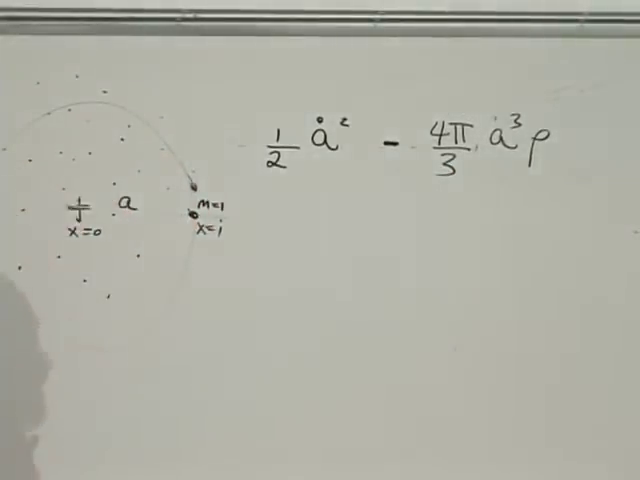
\includegraphics[width=0.78\textwidth]{lecture_03_figure_02.png}\caption{Homogene Kugel mit Mittelpunkt \(x=0\), eine komovierende Galaxie bei \(x=1\) und die Newtonsche Energiebilanz für \(a(t)\).}\end{figure}

Nur die Materie innerhalb der Kugel mit Radius \(a(t)\) trägt zur Gravitationskraft auf das Teilchen bei \(x=1\) bei. Wir setzen die Masse dieses Teilchens gleich eins. Seine kinetische Energie ist
\begin{equation}
\frac{1}{2}\dot a^2.
\end{equation}
Die innerhalb der Kugel eingeschlossene Masse beträgt
\begin{equation}
M_{\mathrm{enc}}=\frac{4\pi}{3}a^3\rho,
\end{equation}
Die gravitative potenzielle Energie ist daher
\begin{equation}
-\frac{G M_{\mathrm{enc}}}{a}
=
-\frac{4\pi G}{3}a^2\rho.
\end{equation}\editorialnote{Zum Vorlesungszeitpunkt 00:05:30 sind an der Tafel der kinetische Term und der von der Dichte abhängige Potenzialterm klar zu erkennen. Der hier notierte vollständige Koeffizient ergibt sich aus der mündlichen Herleitung.}

Aus der Energieerhaltung folgt
\begin{equation}
\frac{1}{2}\dot a^2-\frac{4\pi G}{3}a^2\rho=\text{const}.
\end{equation}
Die Konstante wird dann als \(-k\) geschrieben. Dabei gilt der übliche Vorbehalt: Die Standardnormierung legt diese Schreibweise streng genommen erst fest, nachdem die Gleichung mit \(2\) multipliziert wurde. In der Standardform lautet sie
\begin{equation}
\dot a^2=\frac{8\pi G}{3}a^2\rho-k,
\end{equation}
und Division durch \(a^2\) ergibt
\begin{equation}
\left(\frac{\dot a}{a}\right)^2=\frac{8\pi G}{3}\rho-\frac{k}{a^2}.
\end{equation}
Dies ist die Friedmann-Gleichung in der Form, die in der gesamten Diskussion verwendet wird.

\begin{figure}[ht]\centering
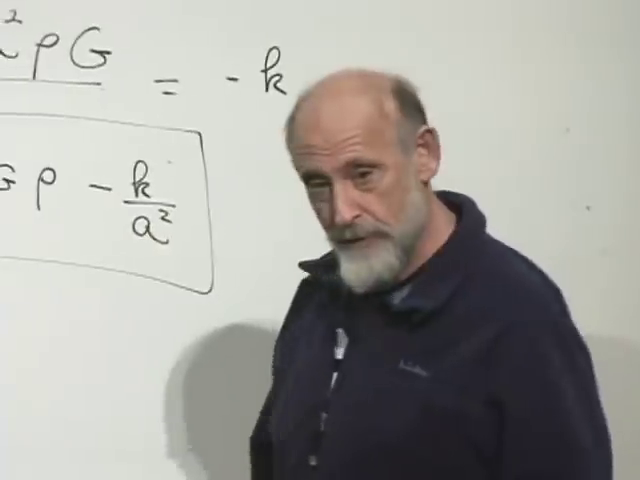
\includegraphics[width=0.56\textwidth]{lecture_03_figure_03.png}\caption{Der Krümmungsbeitrag \(-k/a^2\), isoliert in der Friedmann-Gleichung.}\end{figure}

Der Krümmungsterm ist empirisch sehr nahe bei null; so nahe, dass es auf dieser Betrachtungsebene eine sehr gute Näherung ist, ihn einfach zu vernachlässigen. Er hängt zwar mit der Krümmung des Raumes zusammen, ist hier aber beobachtungsseitig zu klein, als dass sich auch nur sein Vorzeichen bestimmen ließe.

Dieselbe Gleichung ergibt sich auch aus der allgemeinen Relativitätstheorie. Schematisch lautet die Zeit-Zeit-Komponente der Einsteinschen Gleichung
\begin{equation}
R_{00}-\frac{1}{2}g_{00}R \propto T_{00}.
\end{equation}
\editorialnote{Hier wird nur die Tensorstruktur angegeben, nicht der genaue numerische Gesamtkoeffizient.}
Bei einer expandierenden homogenen Metrik ergibt die geometrische Seite die Kombination aus \(\dot a/a\) und \(k/a^2\), während die Materieseite die Energiedichte liefert. An dieser Stelle sagen das Newtonsche Argument und die Einsteinsche Gleichung dasselbe aus.

Damit ändert sich auch die Bedeutung von \(\rho\). Von nun an ist es besser, \(\rho\) als Energiedichte zu bezeichnen. Für langsam bewegte Materie im komovierenden Bezugssystem ist das einfach die Ruheenergiedichte.

\section{Materiedominierte Epoche}

Nehmen wir nun an, dass die Energiedichte von Materie getragen wird, die im komovierenden Bezugssystem ruht. Betrachten wir einen Würfel mit einer Koordinatenlänge von einer Einheit. Seine physikalischen Seitenlängen betragen \(a(t)\), sein physikalisches Volumen also \(a^3(t)\). Wenn die Masse-Energie in diesem komovierenden Würfel \(M\) beträgt und sich die Materie mit der Strömung bewegt, statt die Begrenzung zu überqueren, gilt
\begin{equation}
\rho_m=\frac{M}{a^3}.
\end{equation}

Dies ist der materiedominierte Fall. In dieser Idealisierung ruhen die Teilchen in der Box, daher setzen wir die Temperatur und den Druck gleich null. Druck würde Teilchen erfordern, die die Begrenzung der Box überqueren.

Mit \(k\approx 0\) wird die Gleichung zu
\begin{equation}
\left(\frac{\dot a}{a}\right)^2=\frac{8\pi G}{3}\frac{M}{a^3}.
\end{equation}
Wir versuchen einen Potenzansatz:
\begin{equation}
a(t)=Ct^p.
\end{equation}
Dann gilt
\begin{equation}
\frac{\dot a}{a}=\frac{p}{t},
\end{equation}
Die linke Seite skaliert also wie \(t^{-2}\), die rechte Seite dagegen wie \(t^{-3p}\). Der Vergleich der Potenzen ergibt
\begin{equation}
3p=2,
\qquad
p=\frac{2}{3}.
\end{equation}
Folglich gilt
\begin{equation}
a(t)\propto t^{2/3}.
\end{equation}
Mit dem Koeffizienten erhält man
\begin{equation}
C^3=6\pi G M.
\end{equation}

Entscheidend an der Lösung ist das Potenzgesetz. Ein materiedominiertes Universum expandiert mit der Zweidrittelpotenz der Zeit, nicht linear. Dieses Gesetz beschreibt eine lange Zwischenphase, die ungefähr \(10^5\) Jahre nach dem Urknall beginnt und einige Milliarden Jahre später endet. Das heutige Universum ist nicht im wörtlichen Sinn materiedominiert, denn inzwischen dominiert die Dunkle Energie. Gewöhnliche Materie und ein großer Abschnitt der kosmischen Geschichte lassen sich jedoch so beschreiben.

\section{Strahlungsdominierte Epoche}

Zu noch früheren Zeiten wurde die Energiedichte von Strahlung dominiert. Der Grund ist einfach: Das Universum enthält enorm viele Photonen, ungefähr \(10^9\) Photonen auf jedes Proton. Wird das Universum komprimiert, gewinnen diese Photonen an Energie.

Ein Photon hat keine Ruhemasse, aber es besitzt Energie. Seine Energie ist
\begin{equation}
E_\gamma=h\nu=\frac{hc}{\lambda}.
\end{equation}
Entscheidend ist die Annahme, dass sich die Photonenwellenlängen bei der Expansion des Universums mit ausdehnen:
\begin{equation}
\lambda\propto a.
\end{equation}
Eine Welle in einer Box veranschaulicht das gut. Wenn die Box größer wird, wächst die Wellenlänge der Mode mit ihr. Dieselbe Vorstellung wenden wir hier auf das expandierende Universum an.

Da \(\lambda\propto a\), skaliert die Energie jedes Photons wie
\begin{equation}
E_\gamma\propto a^{-1}.
\end{equation}
Betrachten wir erneut eine komovierende Einheitsbox. Photonen treten ein und aus, aber im Mittel bleibt ihre Anzahl darin konstant. Daher skaliert auch die gesamte Photonenergie in der Box wie \(a^{-1}\). Teilt man durch das physikalische Volumen \(a^3\), so skaliert die Energiedichte der Strahlung wie
\begin{equation}
\rho_r\propto a^{-4}.
\end{equation}

Dieser zusätzliche Faktor \(a^{-1}\) macht den ganzen Unterschied aus. Materie verdünnt sich durch die Expansion des Universums. Strahlung verdünnt sich aus demselben Grund und zusätzlich dadurch, dass jedes Photon rotverschoben wird.

Die Friedmann-Gleichung für ein strahlungsdominiertes Universum lautet daher
\begin{equation}
\left(\frac{\dot a}{a}\right)^2=\frac{8\pi G}{3}\frac{M_r}{a^4}.
\end{equation}\editorialnote{In der mündlichen Diskussion wird das Symbol \(M\) für diese neue Konstante wiederverwendet. Der Index \(r\) wird hier nur hinzugefügt, um Verwechslungen mit dem Materiefall zu vermeiden.}

Wir verwenden denselben Ansatz \(a(t)=Ct^p\). Die linke Seite skaliert erneut wie \(t^{-2}\), die rechte Seite dagegen wie \(t^{-4p}\). Der Vergleich der Potenzen ergibt
\begin{equation}
4p=2,
\qquad
p=\frac{1}{2}.
\end{equation}
Also gilt
\begin{equation}
a(t)\propto t^{1/2}.
\end{equation}
Mit dem Koeffizienten erhält man
\begin{equation}
C^4=\frac{32\pi G}{3}M_r.
\end{equation}

\begin{classroomqa}\lecturetimestamp{00:35:41}\audiencequestion{Warum steht da ein \(G\)}\lecturerresponse{Weil die Energiedichte gravitativ wirkt, nicht allein die Ruhemasse. Bei langsam bewegter Materie ist der Unterschied leicht zu übersehen, aber Photonen machen ihn deutlich: Sie haben keine Ruhemasse und wirken trotzdem gravitativ.}\end{classroomqa}

Eine Box voller Strahlung veranschaulicht den Punkt. Drückt man auf eine mit Photonen gefüllte Box, so wird nach deren Beschleunigung die Wand, die sich auf die Photonen zubewegt, stärker getroffen als die Wand, die sich von ihnen entfernt. Daher muss man stärker gegen den Strahlungsdruck drücken. Die Box hat somit zusätzliche Trägheit, und nach dem Äquivalenzprinzip bedeutet diese zusätzliche Trägheit auch zusätzliche gravitative Masse. Darauf beruht hier das Argument mit der Photonenbox: Energie wirkt gravitativ.

\begin{classroomqa}\lecturetimestamp{00:38:11}\audiencequestion{Lässt sich eine dieser Gleichungen mit einem \(a\) lösen, das mit der Zeit abnimmt?}\lecturerresponse{Ja. Nimmt man den Krümmungsterm \(k/a^2\) wieder hinzu, gibt es Lösungen, bei denen das Universum zunächst expandiert und sich anschließend wieder zusammenzieht. Das scheint unserem Universum nicht zu entsprechen, aber die Gleichung lässt eine solche Entwicklung zu.}\end{classroomqa}

\begin{classroomqa}\lecturetimestamp{00:38:44}\audiencequestion{Was ist aus der Energieerhaltung geworden?}\lecturerresponse{Nimmt man den Term \(k\) wieder hinzu und multipliziert die Gleichung mit \(a^2\) zurück, ist die kosmologische Gleichung genau das Erhaltungsgesetz. Materie oder Strahlung auf der einen Seite ist nur ein Teil der Bilanz. Die Expansion trägt den kinetischen und gravitativen Anteil bei, und die Gesamtbilanz bleibt erhalten.}\end{classroomqa}

\section{Materie und Strahlung zusammen}

In der realen Kosmologie gibt es sowohl Materie als auch Strahlung. Ihre Dichten skalieren unterschiedlich:
\begin{equation}
\rho_m\propto a^{-3},
\qquad
\rho_r\propto a^{-4}.
\end{equation}
Bei kleinen \(a\) dominiert also die Strahlung. Bei großen \(a\) dominiert die Materie. Rückwärts betrachtet muss das frühe Universum daher strahlungsdominiert gewesen sein.

\begin{figure}[ht]\centering
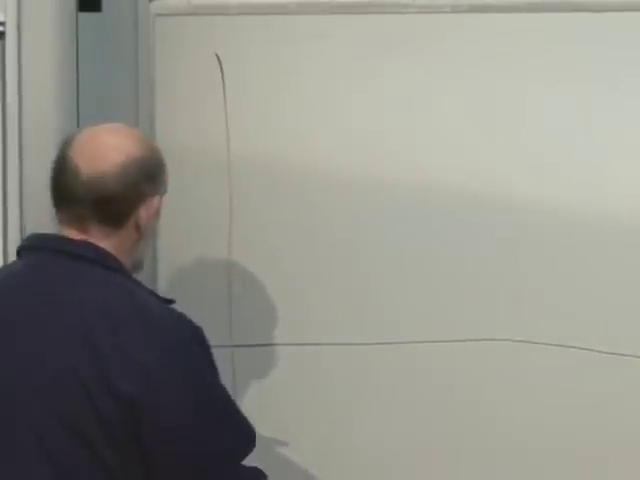
\includegraphics[width=0.68\textwidth]{lecture_03_figure_05.png}\caption{Achsen zum Vergleich der Materie- und Strahlungsenergiedichte als Funktionen des Skalenfaktors.}\end{figure}

\editorialnote{Zum Vorlesungszeitpunkt 00:44:45 sind zu Beginn der Vergleichsdiagramms an der Tafel nur die Achsen zu sehen. Die unmittelbar danach besprochenen Materie- und Strahlungskurven werden im Text beschrieben, aber hier nicht erneut eingezeichnet.}

Die Materiekurve fällt wie \(a^{-3}\). Die Strahlungskurve fällt wie \(a^{-4}\). Beide divergieren für \(a\to 0\), aber dort steigt die Strahlungskurve schneller an, sodass sich die beiden Kurven bei einem Gleichheits-Skalenfaktor schneiden. Eine grobe Schätzung datiert diesen Übergang auf ungefähr \(10^4\) Jahre, vielleicht etwas später.

Derselbe Sachverhalt lässt sich in einem Diagramm von \(a(t)\) gegen \(t\) darstellen. Früh verhält sich die Expansion wie \(t^{1/2}\), später wie \(t^{2/3}\). Der Übergang erfolgt nicht sprunghaft, sondern kontinuierlich über einen relativ engen Zeitbereich.

\begin{classroomqa}\lecturetimestamp{00:44:04}\audiencequestion{Geht die Potenz \(p\) mit dem Alter des Universums kontinuierlich von \(1/2\) zu \(2/3\) über?}\lecturerresponse{Ja. Sie springt nicht. Der Übergang ist kontinuierlich, obwohl er sich über einen ziemlich engen Zeitbereich erstreckt.}\end{classroomqa}

\section{Temperatur, Rekombination und letzte Streuung}

Als Nächstes betrachten wir die Temperatur. Wenn die Energie eines typischen Photons wie \(a^{-1}\) skaliert, dann tut dies auch die Temperatur des Strahlungsbads:
\begin{equation}
T\propto a^{-1}.
\end{equation}
Verdoppelt sich \(a\), halbiert sich die Temperatur.

Setzen wir die heutige Photonentemperatur mit etwa \(3\,\mathrm K\) und die Ionisierungstemperatur mit etwa \(3000\,\mathrm K\) an, ungefähr der Temperatur der Sonnenoberfläche. Dann gilt
\begin{equation}
\frac{a_{\mathrm{today}}}{a_{\mathrm{ion}}}\sim 10^3.
\end{equation}
Mit dem Gesetz \(a\propto t^{2/3}\) für die materiedominierte späte Epoche ergibt sich
\begin{equation}
\left(\frac{t_{\mathrm{today}}}{t_{\mathrm{ion}}}\right)^{2/3}\sim 10^3,
\end{equation}
also
\begin{equation}
\frac{t_{\mathrm{today}}}{t_{\mathrm{ion}}}\sim 1000^{3/2}\sim 3\times 10^4.
\end{equation}
Setzen wir für diese Abschätzung das Alter des Universums mit \(10^{10}\) Jahren an, erhalten wir
\begin{equation}
t_{\mathrm{ion}}\sim 3\times 10^5\ \mathrm{years}.
\end{equation}

Dies ist die Epoche, in der Wasserstoff und Helium aufhören, vollständig ionisiert zu sein. Davor ist das Universum ein heißes Plasma. Warum ist ein Plasma undurchsichtig? Weil freie Ladungen stark auf elektromagnetische Wellen reagieren. Das elektrische Feld treibt die Ladungen hin und her; das Medium verhält sich wie ein Leiter, und Leiter sind undurchsichtig. Darin liegt die einschlägige Analogie zur Sonnenoberfläche.

Sobald das Universum so weit abgekühlt ist, dass Elektronen mit Atomkernen rekombinieren, entstehen gewöhnliche neutrale Atome und das Universum wird deutlich transparenter. Der Übergang ist nicht unendlich scharf. Es handelt sich um einen unscharfen Ort oder ein unscharfes Zeitintervall, aber für die Kosmologie ist er scharf genug, um als Oberfläche der letzten Streuung bezeichnet zu werden.

Wer nach außen blickt, blickt in der Zeit zurück. Nahe Galaxien zeigen die jüngere Vergangenheit. Weiter entfernte Galaxien zeigen frühere Zeiten. Weit genug entfernt trifft jede Sichtlinie auf die Epoche, in der das Universum noch ionisiert und undurchsichtig war. Elektromagnetische Strahlung kann nichts zeigen, was davor liegt.

Andere Boten könnten prinzipiell noch frühere Zeiten sondieren. Neutrinos sind elektrisch neutral und würden früher entkoppeln. Gravitonen würden, falls sie sich je beobachten ließen, aus noch früheren Epochen stammen. Doch dieselbe schwache Wechselwirkung, die es ihnen ermöglichen würde, das frühe Plasma zu durchdringen, macht sie auch extrem schwer nachweisbar.

Wenn das Universum einst in alle Richtungen so heiß wie die Sonnenoberfläche war, warum blendet uns der Himmel dann nicht? Weil sich die Oberfläche der letzten Streuung von uns entfernt und die von dort eintreffenden Photonen ungefähr um denselben Faktor \(10^3\) rotverschoben wurden, der \(3000\,\mathrm K\) von \(3\,\mathrm K\) unterscheidet. Bei uns kommt Mikrowellenstrahlung an, kein sichtbares Sonnenlicht.

\begin{classroomqa}\lecturetimestamp{01:03:51}\audiencequestion{Können unsere Teleskope also nicht weiter zurückblicken als bis ungefähr \(300{,}000\) Jahre?}\lecturerresponse{Mit elektromagnetischen Teleskopen nicht. Davor war das Universum ionisiert und undurchsichtig. Andere Boten könnten zumindest prinzipiell frühere Epochen sondieren.}\end{classroomqa}

\begin{classroomqa}\lecturetimestamp{01:08:43}\audiencequestion{Wenn Sie von der Temperatur eines Photons sprechen, meinen Sie die Temperatur eines schwarzen Körpers mit diesem Strahlungsmaximum. Aber die hängt doch nicht linear von der Wellenlänge ab, oder?}\lecturerresponse{Richtig. Die Temperatur entspricht im Wesentlichen der Energie eines typischen Photons; für ein Photon skaliert sie daher umgekehrt proportional zur Wellenlänge. Das Gesetz \(T^4\) bezieht sich auf die Energiedichte, nicht auf die Energie eines einzelnen Photons. Es berücksichtigt sowohl die Energie pro Photon als auch die Anzahl der Photonen pro Volumeneinheit; die Teilchendichte skaliert wie \(T^3\).}\end{classroomqa}

Somit gilt
\begin{equation}
n_\gamma\propto T^3,
\qquad
\rho_\gamma\propto T^4.
\end{equation}

\section{Dunkle Materie aus Rotationskurven}

Dunkle Materie kommt über galaktische Rotationskurven ins Spiel. Sie wurde nicht aus der großräumigen Friedmann-Gleichung abgeleitet, sondern aus astronomischen Beobachtungen auf galaktischen Skalen.

Beginnen wir mit dem einfachsten Newtonschen Problem: Ein leichter Körper der Masse \(m\) umläuft eine zentrale Masse \(M\) im Abstand \(r\). Die Gravitationskraft beträgt
\begin{equation}
\frac{GMm}{r^2},
\end{equation}
und die Zentripetalbeschleunigung ist \(v^2/r\). Nach dem Newtonschen Gesetz gilt
\begin{equation}
m\frac{v^2}{r}=\frac{GMm}{r^2}.
\end{equation}
Kürzen wir \(m\) und multiplizieren mit \(r\), erhalten wir
\begin{equation}
v(r)=\sqrt{\frac{GM}{r}}.
\end{equation}
Wenn sich die gravitative Masse also nahe dem Zentrum konzentriert, nimmt die Umlaufgeschwindigkeit wie \(r^{-1/2}\) ab.

Das wäre zu erwarten, wenn die Masse der Lichtverteilung folgte. Der größte Teil der sichtbaren Materie einer Galaxie liegt nahe ihrem Kern, sodass sich äußere Sterne dann ähnlich wie Planeten in den äußeren Bereichen des Sonnensystems verhalten würden. Astronominnen und Astronomen bestimmen die Umlaufgeschwindigkeiten, indem sie die Dopplerverschiebungen auf gegenüberliegenden Seiten einer nahen Galaxie messen und dabei die sich auf uns zubewegende Seite mit der sich von uns wegbewegenden vergleichen, nachdem sie die gemeinsame Rezessionsbewegung der ganzen Galaxie herausgerechnet haben. Die gemessenen Umlaufgeschwindigkeiten bleiben bis zu großen Radien ungefähr konstant.

Ersetzen wir also die zentrale Masse \(M\) durch die eingeschlossene Masse \(M(r)\):
\begin{equation}
\frac{v^2}{r}=\frac{G M(r)}{r^2}.
\end{equation}
Ist \(v(r)\) annähernd konstant, dann gilt
\begin{equation}
M(r)\propto r.
\end{equation}
Mit anderen Worten: Die gravitative Masse nimmt mit dem Radius weiter zu, selbst dort, wo das sichtbare Licht es nicht tut.

Nehmen wir nun, der Einfachheit halber wie in der Diskussion, an, dass die Massenverteilung ungefähr kugelsymmetrisch ist. Dann gilt
\begin{equation}
M(R)=\int_0^R 4\pi r^2\rho(r)\,dr.
\end{equation}
Wenn \(M(R)\propto R\), ergibt die Ableitung nach \(R\)
\begin{equation}
4\pi R^2\rho(R)\propto 1,
\end{equation}
und somit
\begin{equation}
\rho(r)\propto \frac{1}{r^2}.
\end{equation}

\begin{classroomqa}\lecturetimestamp{01:28:18}\audiencequestion{Es sieht so aus, als müsste die Dichte wie \(1/r^2\) abnehmen. Gibt es dafür einen Grund?}\lecturerresponse{Aus der beobachteten flachen Rotationskurve folgt \(M(R)\propto R\); durch Ableiten erhält man dann \(\rho(r)\propto 1/r^2\). Darüber hinaus wird hier keine einfache Erklärung aus ersten Prinzipien beansprucht; detaillierte Simulationen leisten einen großen Teil der Arbeit.}\end{classroomqa}

Die belastbare Schlussfolgerung lautet, dass eine Galaxie wesentlich mehr gravitative Masse enthält, als allein die leuchtende Materie vermuten ließe: mehrere Male mehr, in der hier verwendeten Schätzung ungefähr eine Größenordnung mehr. Die sichtbare Galaxie liegt in einem viel größeren dunklen Halo.

Was hindert gewöhnliches Gas daran, in einem solchen diffusen Zustand zu verbleiben? Dissipation. Eine Gaswolke zieht sich zusammen, weil Stöße, reibungsähnliche Prozesse und Strahlung ihr Energie entziehen können. Dunkle Materie strahlt offenbar kaum und ist nahezu kollisionsfrei. Die Gravitation kann sie nach innen ziehen und potenzielle Energie in kinetische Energie umwandeln, doch ohne effiziente Dissipation kollabiert sie nicht zu den kompakten leuchtenden Strukturen, die gewöhnliche Materie bildet. Die kinetische Energie hält den Halo ausgedehnt.

Anschließend werden einige Alternativen mit Vorsicht erörtert. Neutrinos seien zu schnell, um sich auf galaktischen Skalen auf diese Weise zu verhalten. Ein Halo aus gewöhnlichem Wasserstoff würde die Nukleosynthese im frühen Universum erheblich stören. Auch Schwarze Löcher aus gewöhnlicher Materie werden als problematisch erwähnt, denn sie würden zu viel gewöhnliche Materie im frühen Universum voraussetzen und Fragen zur Gravitationslinsenwirkung aufwerfen. Mehr wird an dieser Stelle nicht behauptet.

Der Halo wird weder als dünne Schale noch als Torus beschrieben. Er ist eine ungefähr kugelförmige, inhomogene Materieverteilung: dichter zum Zentrum hin und nach außen allmählich abfallend.

\begin{classroomqa}\lecturetimestamp{01:53:12}\audiencequestion{Meinen Sie den Bullet-Cluster?}\lecturerresponse{Ja. Das Röntgengas zeigt die gewöhnliche Materie, während Gravitationslinsen die gesamte gravitative Masse sichtbar machen. Bei der Kollision trennen sich diese beiden Verteilungen voneinander. Das ist ein starker Beleg für reale Dunkle Materie und gegen eine bloße Modifikation der Gravitation, die allein an die sichtbare Materie gebunden ist.}\end{classroomqa}

Das ist der abschließende Beobachtungsbefund. Über die genaue Beschaffenheit der Dunklen Materie ist nur sehr wenig bekannt, doch nichts von dem hier Gesagten erfordert ein radikal neues Prinzip. Die konservative Möglichkeit ist schlicht, dass es in der Natur zusätzliche schwach wechselwirkende Teilchen gibt, die bislang nicht identifiziert wurden.
